\documentclass[9pt,twocolumn,twoside,lineno]{pnas-new}
% Use the lineno option to display guide line numbers if required.
% Note that the use of elements such as single-column equations
% may affect the guide line number alignment. 

\usepackage[super]{nth} %adds superscripts for things like 20th

\templatetype{pnasresearcharticle} % Choose template 

\title{The Changing Character of Rainfall in Eastern China, 1951-2007}

% Use letters for affiliations, numbers to show equal authorship (if applicable) and to indicate the corresponding author
\author[a,1]{Jesse Day}
\author[a]{Inez Fung} 
\author[b]{Weihan Liu}

\affil[a]{Department of Earth and Planetary Science, University of California Berkeley, 94720}
\affil[b]{College of Letters and Sciences, University of California Berkeley, 94720}

%\subsection*{Author Affiliations}

%Include department, institution, and complete address, with the ZIP/postal code, for each author. Use lower case letters to match authors with institutions, as shown in the example. Authors with an ORCID ID may supply this information at submission.

% Please give the surname of the lead author for the running footer
\leadauthor{Day} 

% Please add here a significance statement to explain the relevance of your work
\significancestatement{Eastern China experienced a late-twentieth-century change in rainfall known as the ``South Flood-North Drought.'' Permanently altered rainfall in this densely populated region would have severe humanitarian repercussions. We develop an algorithm that identifies elongated patterns in rainfall maps. In summer, these elongated patterns are associated with the well known Meiyu front, and we find that these events are primarily responsible for the increase in rainfall in eastern China. Changes in the frequency of frontal rainfall explain the overall pattern of rainfall changes across 1951-2007, with an uptick in frontal rainfall daily intensity after 1993. In contrast, there is no significant trend in non-frontal rainfall. The classification provides a framework for diagnosis of the relative roles of global warming, aerosols and natural variability in historical rainfall change.}

% Please include corresponding author, author contribution and author declaration information
\authorcontributions{J.D. developed the FREDA algorithm, created the catalog and wrote the manuscript; J.D. and I.F. contributed equally to the interpretation of results; W.L. contributed to algorithm development.}
\authordeclaration{The authors declare no conflict of interest.}
\correspondingauthor{\textsuperscript{1}Corresponding author. Email: jessed@berkeley.edu}

% Keywords are not mandatory, but authors are strongly encouraged to provide them. If provided, please include two to five keywords, separated by the pipe symbol, e.g:
\keywords{East Asian Monsoon|Monsoons|Rainfall|Meiyu Front|New Methods} 

% max word length: 250
\begin{abstract}
The topography and continental configuration of East Asia favor the year-round existence of storm tracks that extend thousands of kilometers from China into the northwestern Pacific Ocean, producing zonally elongated patterns of rainfall that we call ``frontal rain events.'' In spring and early summer (``Meiyu Season''), frontal rainfall intensifies and shifts northward during a series of stages collectively known as the East Asian summer monsoon. Using a new technique called the Frontal Rain Event Detection Algorithm (FREDA), we create a daily catalog of all frontal rain occurrences in East China during 1951-2007, quantify their attributes, and classify all rainfall on each day as either frontal, resulting from large-scale frontal convergence, or non-frontal, produced by local buoyancy, topography or cyclones. Our climatology shows that the East Asian summer monsoon consists of a series of coupled changes in frontal rain event frequency, latitude and daily intensity. Furthermore, decadal changes in the amount and distribution of rainfall in East China are overwhelmingly due to changes in frontal rainfall. We attribute the ``South Flood-North Drought'' pattern observed beginning in the 1980s to changes in the frequency of frontal rain events, while the years 1994-2007 witnessed an uptick in event daily intensity relative to the rest of the study years. This particular signature may reflect the relative impacts of global warming, aerosol loading and natural variability on regional rainfall change, potentially by shifting the East Asian jet stream.
\end{abstract}

\dates{This manuscript was compiled on \today}
\doi{\url{www.pnas.org/cgi/doi/10.1073/pnas.XXXXXXXXXX}}

\begin{document}

% Optional adjustment to line up main text (after abstract) of first page with line numbers, when using both lineno and twocolumn options.
% You should only change this length when you've finalised the article contents.
\verticaladjustment{-2pt}

\maketitle
\thispagestyle{firststyle}
\ifthenelse{\boolean{shortarticle}}{\ifthenelse{\boolean{singlecolumn}}{\abscontentformatted}{\abscontent}}{}

\dropcap{E}astern China receives about 60\% of its precipitation from May to August via the East Asian summer monsoon. The period of peak rainfall lasting from early June to mid-July is called ``Meiyu season'' (lit. ``plum rains,'' referring to the spectacular growth of plum blossoms in central China with the onset of heavy rains). During this time, heavy rainfall occurs in zonal bands resulting from frontal synoptic conditions (the ``Meiyu Front''). The summer meteorology of Japan and Korea also features similar phenomena (the ``Baiu'' and ``Changma'' respectively). The contribution from these frontal rain events leads to a rainfall seasonality in the East Asian monsoon that is unique relative to other monsoon circulations \citep{Ding2005}. More generally, frontal rainfall is observed year-round due to the interplay between the East Asian tropospheric jet and Tibetan Plateau \citep{Molnar2010,Sampe2010,Chen2014}. According to our subsequent analysis, frontal rainfall amounts to over 40\% of yearly total rainfall in much of East China (105$^{\circ}$E-123$^{\circ}$E and 20$^{\circ}$N-40$^{\circ}$N; Figure~\ref{fig:type_climo}).
	 	  	 
	In this study, we analyze frontal rainfall in East China with the Frontal Rain Event Detection Algorithm (FREDA), an algorithm that locates frontal rain events in daily precipitation maps and quantifies attributes such as latitude and daily intensity (daily precipitation accumulation). We apply FREDA to APHRODITE precipitation data from East China to create a catalog of all frontal rain events during 1951-2007 (20,819 days total), and we also classify all rainfall on each day as either frontal or non-frontal. Both the data set and algorithm are described in greater details in the Materials and Methods.
	
	The length of the resulting data set allows us to focus on decadal changes in frontal rainfall. We investigate the ``South Flood-North Drought'' phenomenon reported in East China post-1980 \citep{Hu1997,Gong2002,Nigam2013}, as well as a reported rainfall change between 1994-2007 and 1980-1993 \citep{Wu2010,Kajikawa2012}. While several previous studies have compiled evidence of the variability of the Meiyu front on decadal and centennial timescales \citep{Chen2004,Ge2008,Xu2009}, no prior catalog of frontal rainfall exists that spans multiple decades with daily resolution. We hope that our analysis can clarify the impact of external forcing such as global warming and aerosols on East China rainfall, and that historical links can be used to inform future rainfall projections for the region.
	
%%FIGURE 1 Decadal mean in different rainfall types during different time periods
\begin{figure}[htb]
\centering
\noindent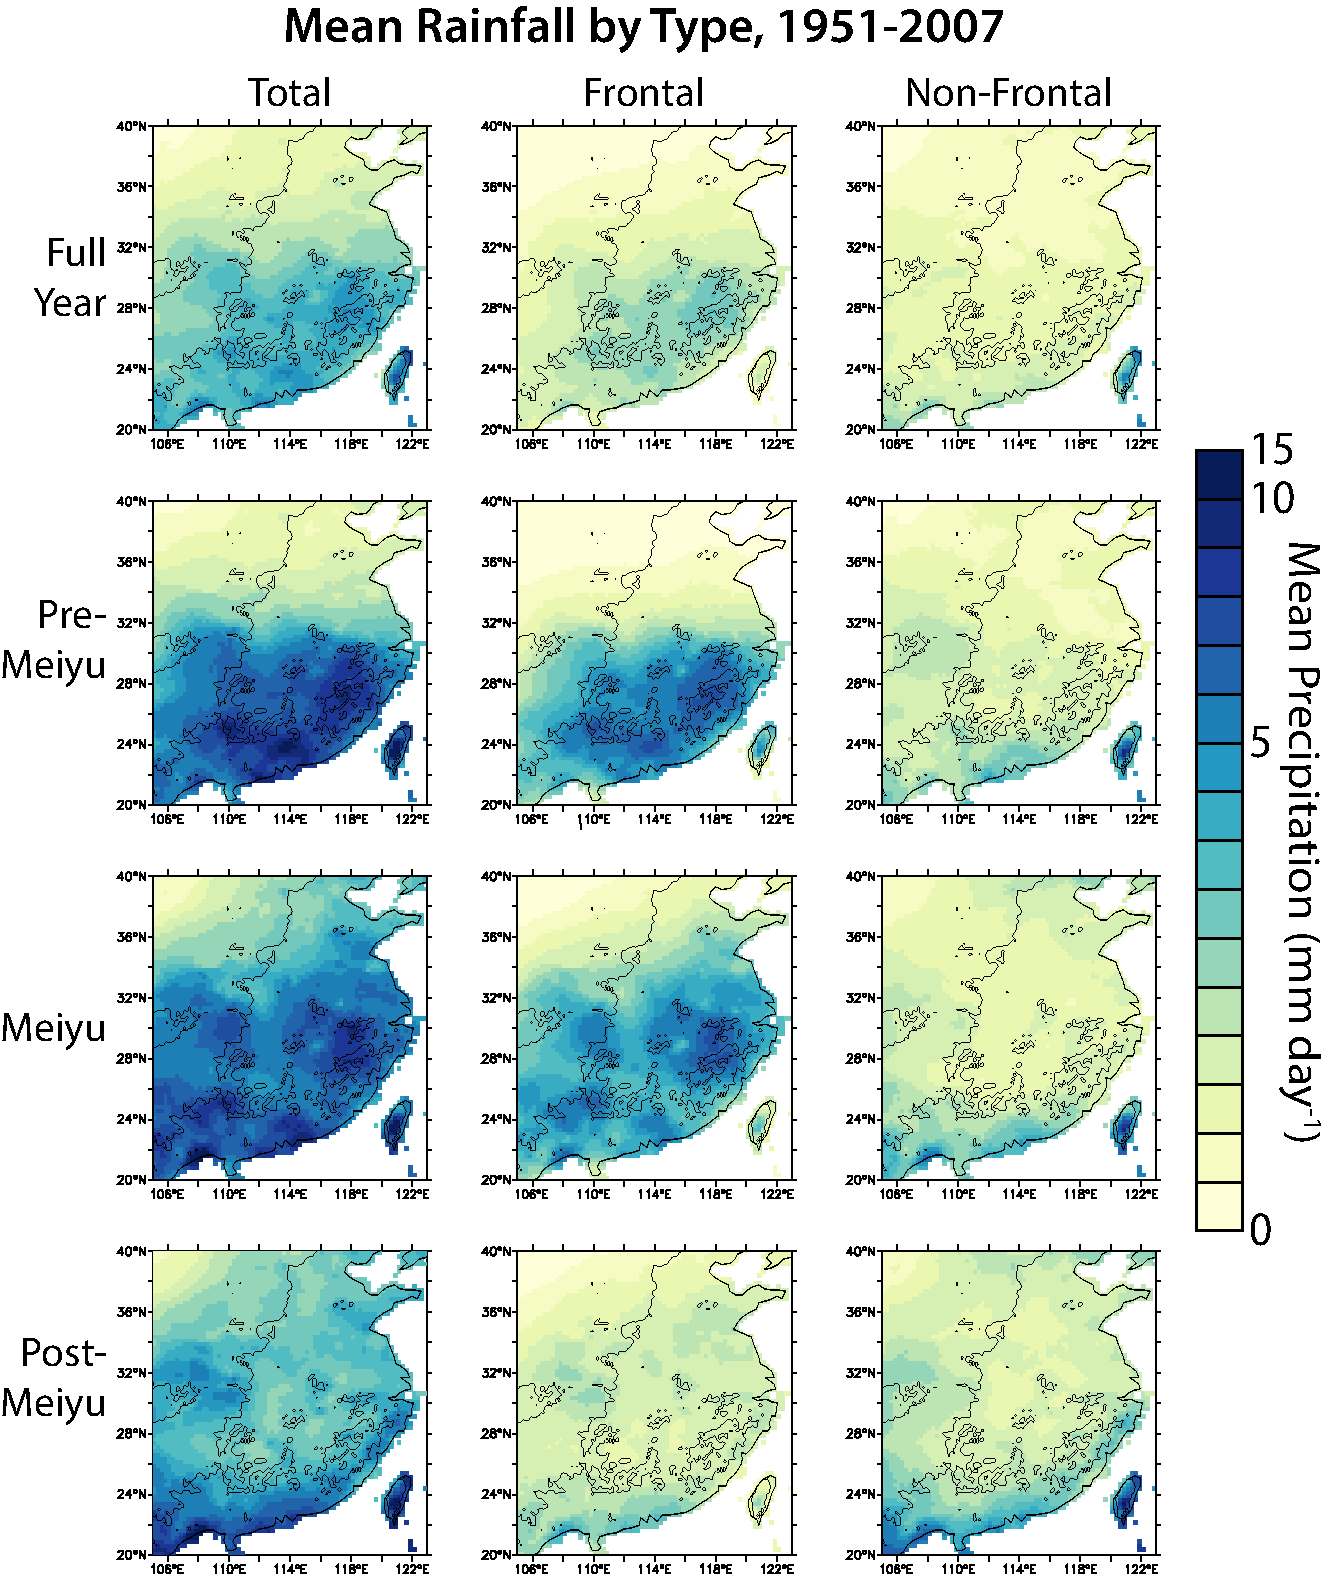
\includegraphics[width=\linewidth]{Figures/type_climo}
\caption{Climatological rainfall, frontal rainfall and non-frontal rainfall for the full year, Pre-Meiyu (days 121-160), Meiyu (days 161-200) and Post-Meiyu (days 201-273). \textit{Frontal} rainfall consists of all rainfall falling within 4$^{\circ}$ of a frontal rain event's axis and rainfall at any other adjacent point exceeding 10 mm day$^{-1}$. \textit{Non-frontal} rainfall includes all rainfall not meeting these criteria. Note that color bar switches from .5 to 1 mm day$^{-1}$ increment past 5 mm day$^{-1}$.}
\label{fig:type_climo}
\end{figure}

\section*{Frontal Rain Event Climatology}

	The mean yearly progression of East China precipitation during 1951-2007 is shown in Figure~\ref{fig:hov_climo}a and can be compared with reference \cite{Ding2005}. Abrupt climatological shifts in rainfall and frontal rain event climatology frequently co-occur. Frontal rain events appear in all months, with maximum frequency and daily intensity in late June (80\%, mean of 31 mm day$^{-1}$) and a minimum in January (10\% and mean daily intensity of 12 mm day$^{-1}$). We define 5 periods of distinct behavior as demarcated in Figure~\ref{fig:hov_climo}, with the Pre-Meiyu, Meiyu and Post-Meiyu equivalent to the three stages of Meiyu rainfall described in reference \cite{Ding2005}:

\begin{enumerate}

\item The Spring Rains (days 60-120, March 1-April 30), previously studied in reference \cite{Tian1998}, marked by frequent but relatively weak frontal rain events (47\% occurrence, 20 mm day$^{-1}$ mean);

\item Pre-Meiyu season (days 121-160, May 1-June 9), during which rainfall and front daily intensity steadily increase (56\% occurrence, 25.5 mm day$^{-1}$ mean);

\item Meiyu season (days 161-200, June 10-July 19) when a remarkable 7-degree northward shift in mean frontal rain event latitude occurs over the course of several weeks, and frontal rain event frequency and daily intensity peaks (66\% occurrence, 28.3 mm day$^{-1}$ mean); 

\item Post-Meiyu season (days 201-273, July 20-September 30), when frontal rain events are less common than during the Spring Rains (42\% occurrence) but double frontal events occur more frequently (28\% chance of observing a secondary event if a primary frontal event is observed); 

\item The Fall Rains (days 274-320, October 1-November 16), when mean frontal rain event latitude begins shifting southward from its northern maximum of 30$^\circ$N, and their frequency decreases to just 27\%.

\end{enumerate}

	These time periods are chosen subjectively, but our subsequent analysis is not dependent on their exact duration. Unlike other monsoonal regions, which tend to be very dry in winter \citep{Wang2002}, Eastern China receives about 40\% of yearly precipitation between September and April. The estimate of onset day of Meiyu season roughly matches  reference \citep{Xu2009}. The Pre-Meiyu to Meiyu and Meiyu to Post-Meiyu transitions both entail rapid northward migrations in preferred location of frontal rainfall (Figure~\ref{fig:type_climo}). During days 160-180, likelihood of observing a rainfall maximizes between 26$^\circ$ and 30$^\circ$N, yet by days 200-220, the same region is less likely than any other latitude to feature a frontal rain event (an 80\% decline in event frequency, and a decline in total rainfall from 7.6 mm day$^{-1}$ to 4.1 mm day$^{-1}$). Maxima of frontal rain event frequency and daily intensity are not always collocated in latitude.

%%FIGURE 2 Hovm�ller diagram of Meiyu latitude occupancy, 1951-2007.
\begin{figure}[htbp]
\centering
\noindent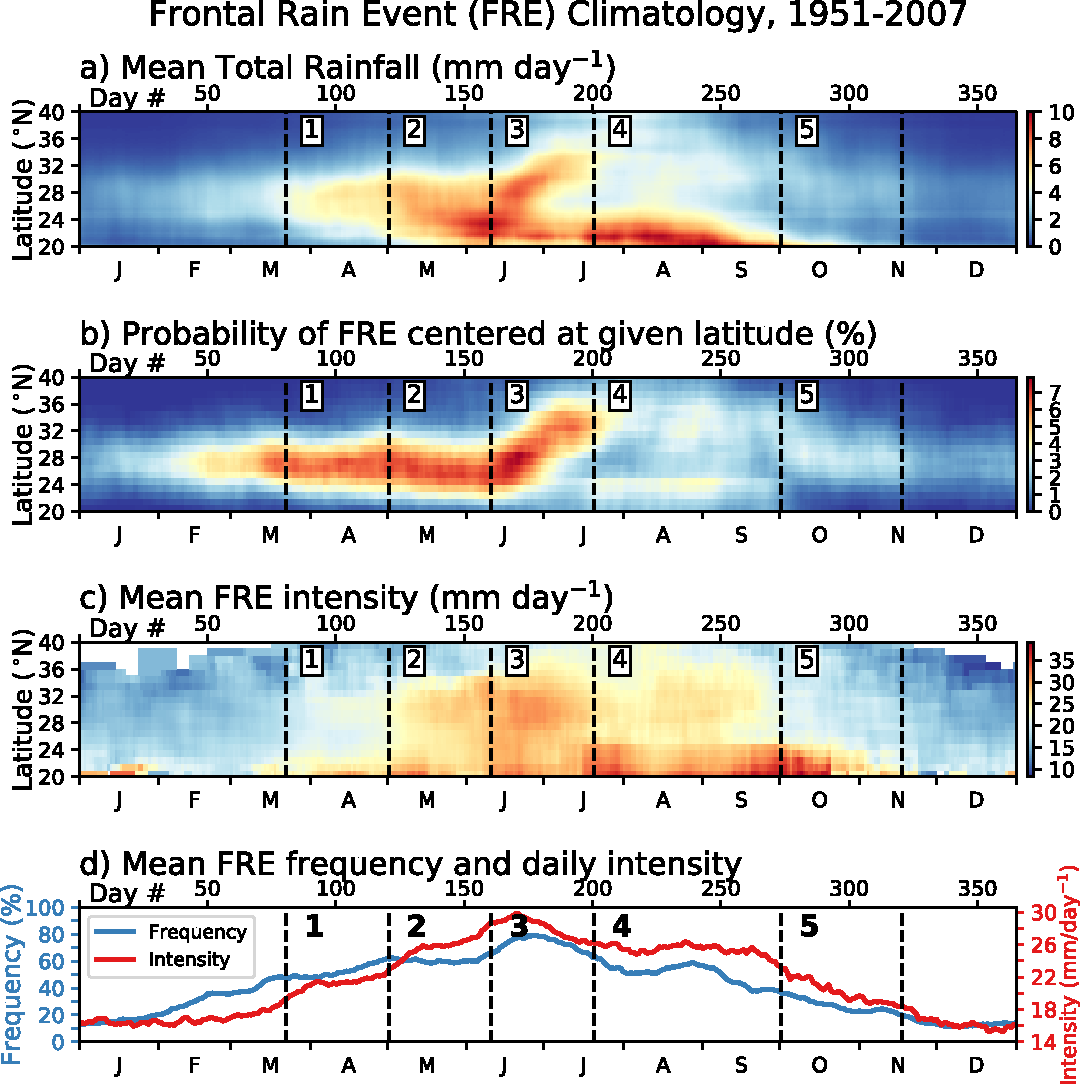
\includegraphics[width=\linewidth]{Figures/PNAS_climo_cropped}
\caption{Climatology of East China rainfall and frontal rain events, 1951-2007, with important time periods marked as follows: 1 - Spring Rains; 2 - Pre-Meiyu; 3 - Meiyu; 4 - Post-Meiyu; 5 - Fall Rains. a) Hovm\"oller diagram of precipitation (100-123$^{\circ}$E longitudinal average); b) Hovm\"oller diagram of probability of observing a FRE at a given latitude, smoothed in time with a 9-day and 2$^{\circ}$-running box filter; c) Mean frontal rain event daily intensity (average of daily intensity of all frontal rain events within 15 days and +/-2.5$^{\circ}$ of latitude); d) Frontal rain event frequency (15-day running mean) and mean daily intensity on each day.}
\label{fig:hov_climo}
\end{figure}
	
	Frontal rain events are generally more probable and stronger during spring than in fall, with notable daily intensity jumps around days 120 and 160. Some periods of heavy rainfall, in particular the August peak over southeastern China (>10 mm day$^{-1}$ around 20$^{\circ}$N), do not correspond to a surge in frontal rain event frequency. Instead, August and September are known as the months when northwestern Pacific typhoons reach mainland China, which tend to leave favorable rainfall conditions in their wake \citep{Chen2007,Chen2011}. The frontal rain events with highest daily intensity occur at low latitudes during October (days 270-300) during peak cyclone season \citep{Liu2003}.
	
%%FIGURE 3 Decadal changes in different rainfall types
\verb|
\begin{figure*}[tp]
\centering
\noindent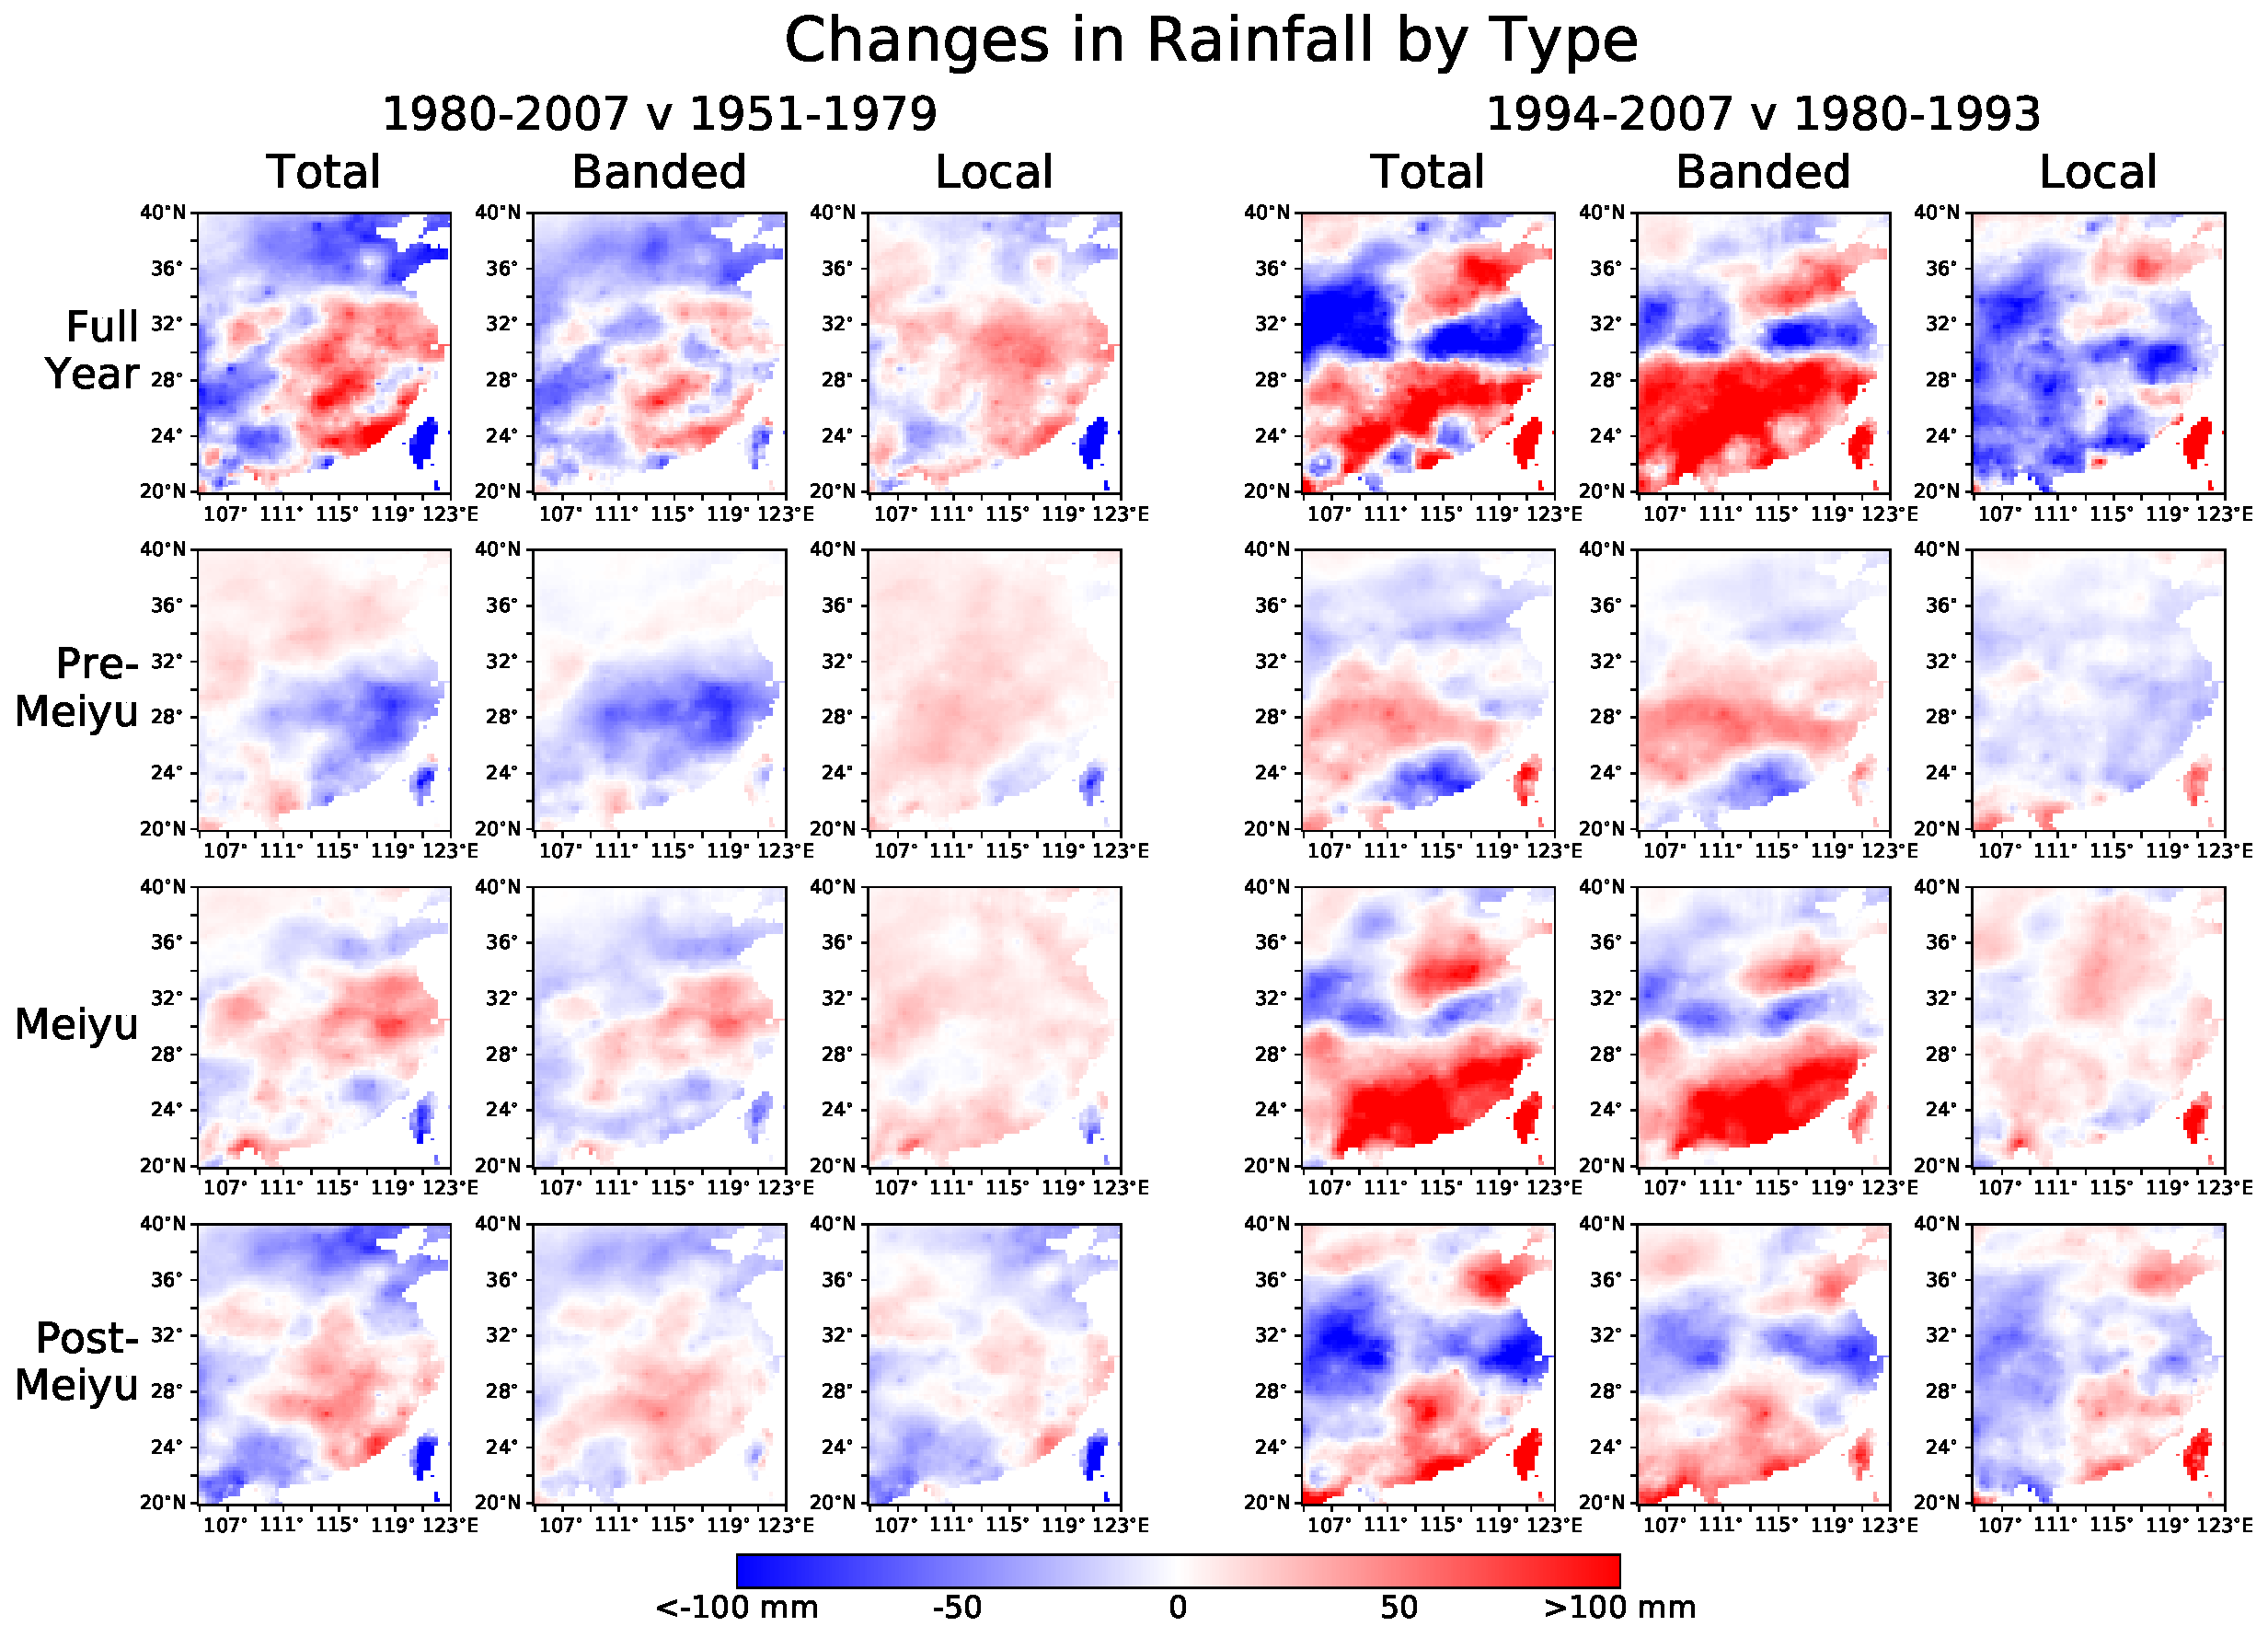
\includegraphics[width=17.8cm]{Figures/changes_by_type}
\caption{Cumulative changes in total, frontal and non-frontal rainfall for full year, Pre-Meiyu (days 121-160), Meiyu (days 161-200) and Post-Meiyu (days 201-273), comparing time periods 1980-2007 to 1951-1979 (left) and 1994-2007 to 1980-1993 (right). \textit{Frontal} rainfall consists of all rainfall falling within 4$^{\circ}$ of a frontal rain event's axis and rainfall at any other adjacent point exceeding 10 mm day$^{-1}$. \textit{Non-Frontal} rainfall includes all rainfall not meeting these criteria.}
\label{fig:type_changes}
\end{figure*}

\subsection*{Frontal versus Non-Frontal Rainfall}	
	
	 FREDA partitions daily rainfall into frontal and non-frontal components. We envision frontal rainfall as resulting from large-scale frontal convergence, while non-frontal rainfall is likely driven locally by buoyancy or topography, or produced by cyclones. The fraction of annual rainfall that is frontal exceeds 60\% in much of Central China, reaching a maximum of 74\% in the vicinity of Jiangxi Province (28$^\circ$N, 116$^\circ$E) (Figures~\ref{fig:type_climo} and S5). Frontal rainfall constitutes the majority of rainfall during the Pre-Meiyu and Meiyu, but not the Post-Meiyu. While frontal rainfall undergoes a dramatic seasonal northward progression from Pre-Meiyu to Post-Meiyu, the spatial distribution of non-frontal rainfall remains largely the same between seasons, with a peak in July-August more typical of other monsoons (Figure S6). Topographic features such as the South China/Qinling mountains and Sichuan Basin anchor regional maxima of non-frontal rainfall. Frontal rainfall only constitutes a noticeable fraction of Taiwanese rainfall during the Pre-Meiyu. In fact, the term Meiyu season as used in Taiwan refers to late May \citep{Chen1994,Xu2009}, not June 10-July 19 as in our study.

%%FIGURE 4 Significance of attribute changes in frontal rain events between decades
\begin{figure}[h]
\centering
\noindent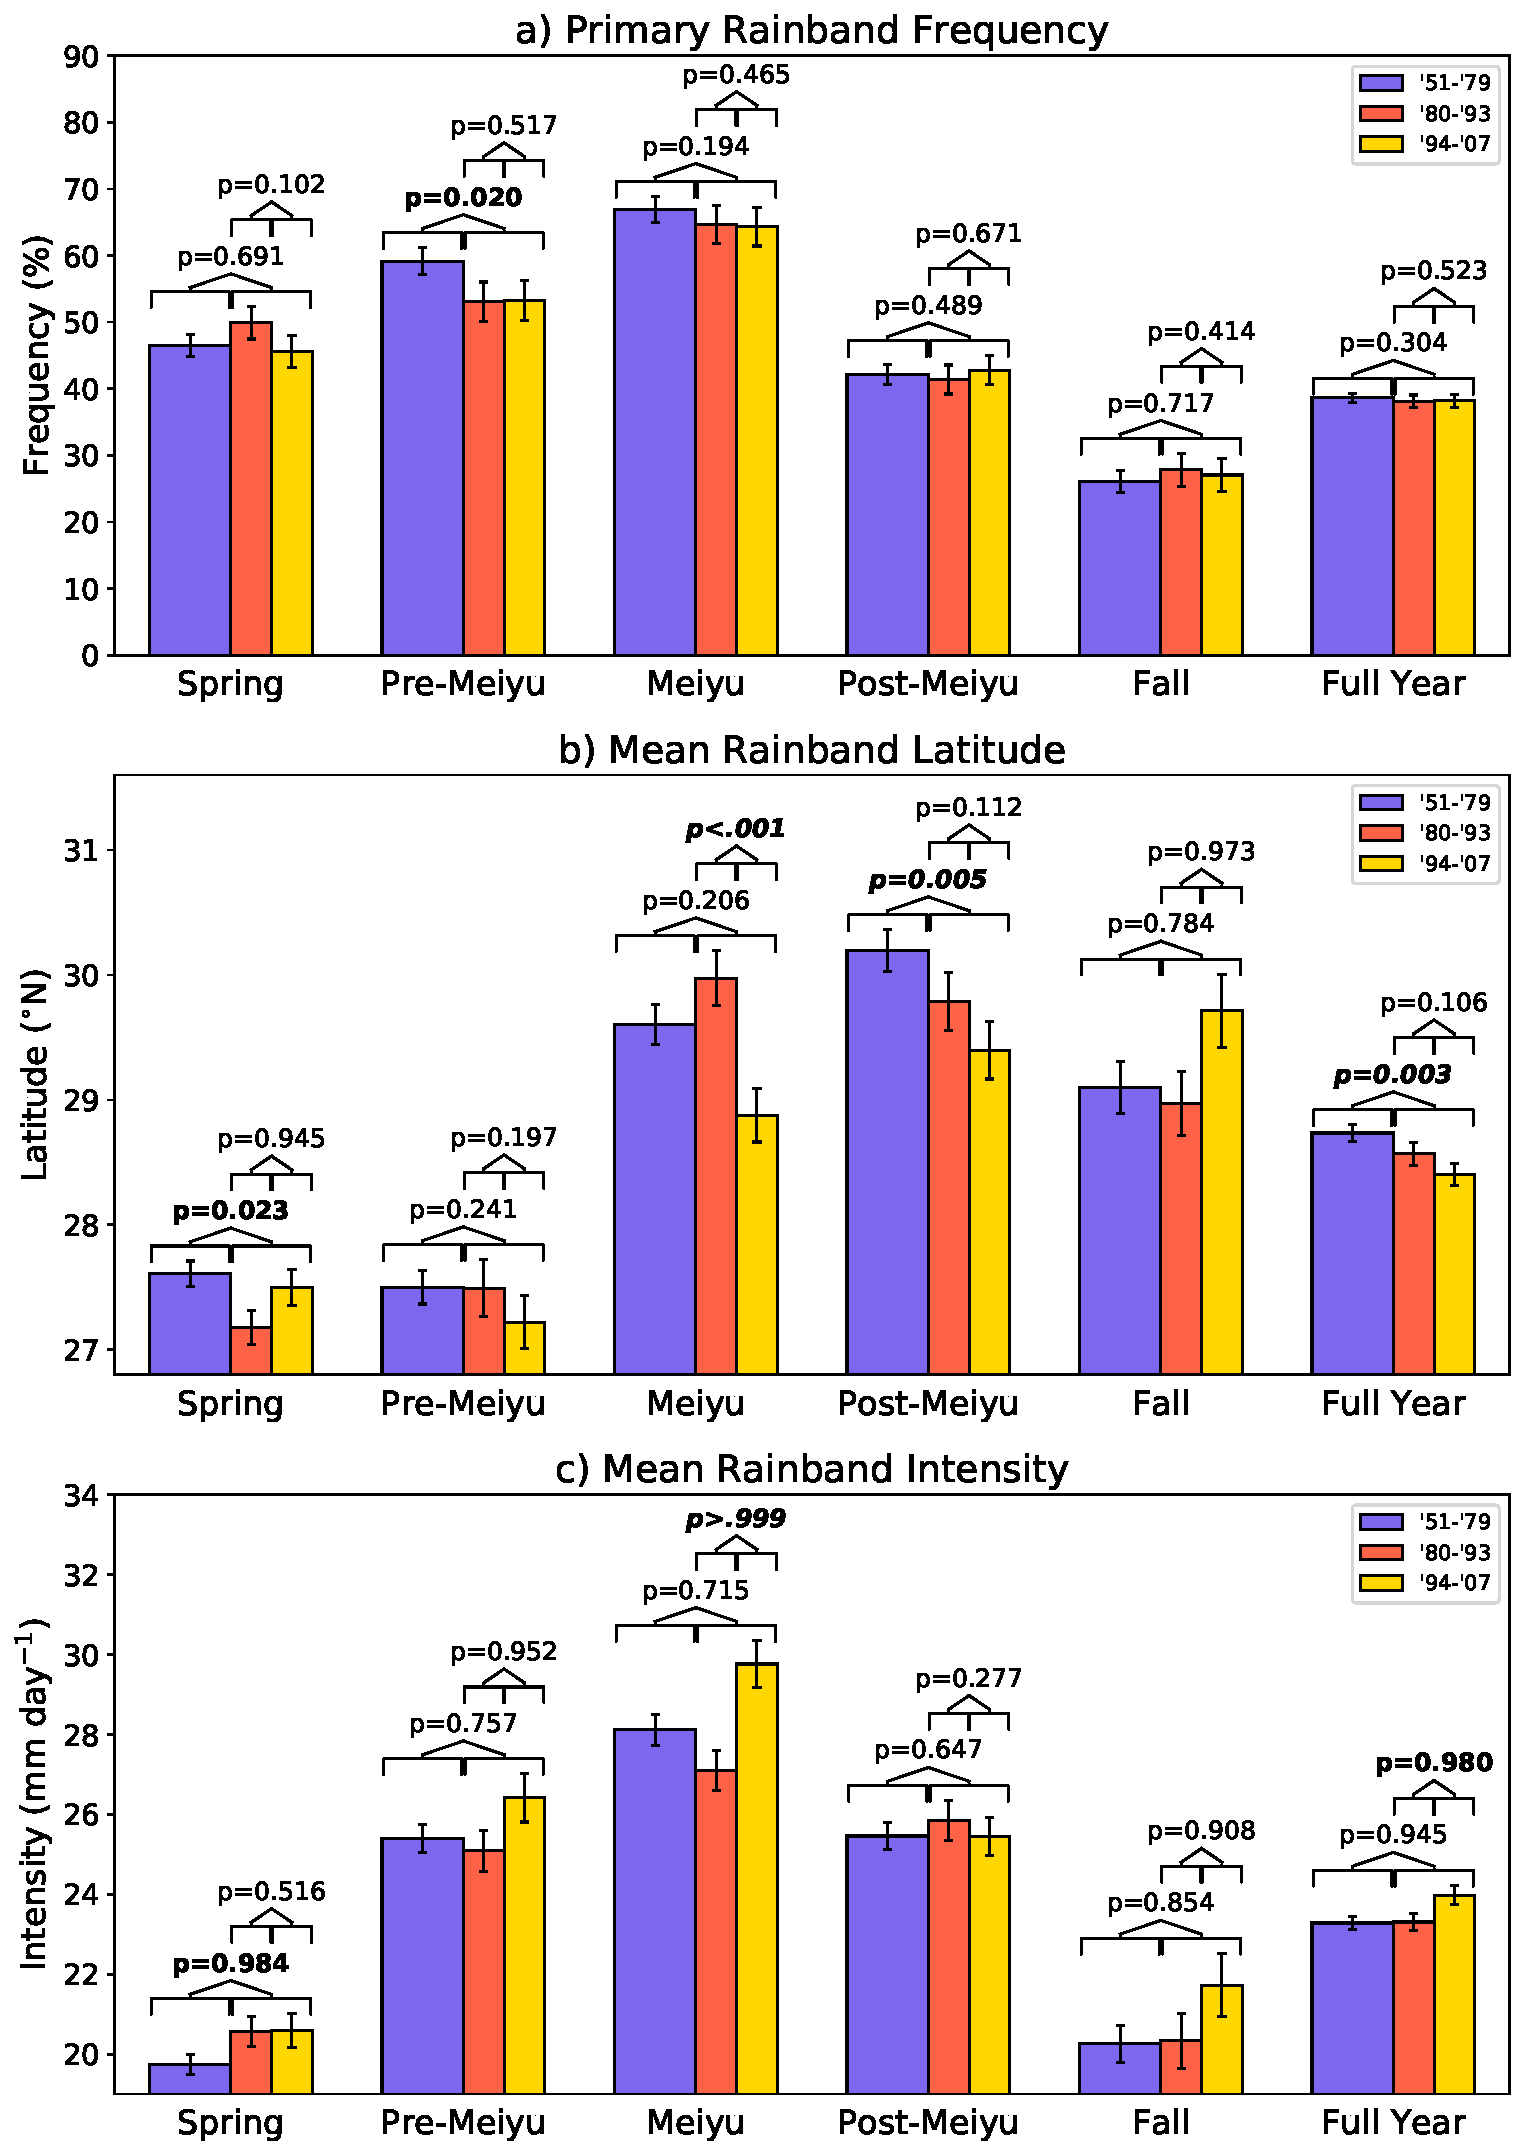
\includegraphics[width=\linewidth]{Figures/bars}
\caption{Significance of decadal changes in a) Frontal rain event frequency, b) Frontal rain event latitude and c) Frontal rain event daily intensity between decades, with comparisons marked for 1980-2007 v 1951-1979 and 1994-2007 v 1980-1993 for each season. The domain is East China (between 105$^{\circ}$E-123$^{\circ}$E and 20$^{\circ}$N-40$^{\circ}$N). Methods of calculating statistical significance are detailed in Supporting Information.}
\label{fig:bars}
\end{figure}	

\section*{Decadal Changes}

	Based on the prior work of other authors, we focus subsequently on comparing 1980-2007 to 1951-1979 and 1994-2007 to 1980-1993. Our results are robust to different choices of years. Spatial changes in rainfall between sets of years for key time periods are shown in Figure~\ref{fig:type_changes} and decomposed into frontal and non-frontal rainfall changes. Figure~\ref{fig:bars} uses bootstrap methods to determine the significance of the overall changes in frontal rain event latitude, frequency and daily intensity during key time periods Finally, Figure~\ref{fig:hov_changes} similarly shows zonally averaged frontal and non-frontal rainfall changes for the entire year in Hovm\"oller plot format, as well as changes in frontal rain event daily intensity and frequency at each latitude.
	
\subsection*{1980-2007 versus 1951-1979}

	Examining the changes in yearly rainfall between 1980-2007 and 1951-1979, a meridional dipole exists between northeastern and southeastern China known as the South Flood-North Drought (Figure~\ref{fig:type_changes}). Pronounced regional shifts are also visible in Taiwan, South Korea and parts of Japan. With the partitioning of these changes into frontal and non-frontal component, two observations can be made: 1) frontal and non-frontal rainfall changes are uncorrelated; 2) changes in total rainfall are predominantly contributed by changes in \textit{frontal} rainfall}, except in Taiwan. In northeastern China, yearly rainfall totals after 1980 decreased due to a decline in frontal rainfall during the Post-Meiyu (July 20-Sep 30). In southeastern China, a corresponding increase in frontal rainfall during the Post-Meiyu is offset by a decline in rainfall during the Pre-Meiyu, such that the yearly change is not statistically significant. Instead, the seasonality of southeastern China rainfall has changed, with later pre-Meiyu onset and more intense Meiyu and Post-Meiyu seasons. Frontal rainfall anomalies are concentrated in summer, when frontal rain events are most frequent. Given these observations, we suggest that frontal and non-frontal rainfall reflect different underlying rainfall mechanisms that have undergone distinct evolutions in recent decades. 
	
	Changes in frontal rainfall can further be attributed to changes in frequency or daily intensity. Changes in frontal rain events in the entire domain between 1980-2007 and 1951-1979 are dominated by changes in \textit{frequency}, while no significant changes in daily intensity are found, contrary to the findings of \cite{Yu2010} (Figure~\ref{fig:hov_changes}). The probability of observing a frontal rain event during the Pre-Meiyu declined from $59.1\% \pm 2.0\%$ to $53.0\% \pm 2.1\%$ ($p=0.020$; Figure~\ref{fig:bars}), leading to a 2 mm day$^{-1}$ daily deficit in frontal rainfall (Figure~\ref{fig:hov_changes}). During the Post-Meiyu, the frequency of frontal rainfall in northeastern China also declined, inducing a southward shift in mean frontal rain event latitude from $33.6^\circ \textrm{N} \pm .3^\circ$ to $32.9^\circ \textrm{N} \pm .3^\circ$ ($p=.005$; Figure~\ref{fig:bars}). If we repeat the analysis only for frontal rain events north of 27$^\circ$N (southeastern China is subject to typhoons during the post-Meiyu, which obey different dynamics and may skew statistics), a p-value of $p=.0003$ is obtained. Kolmogorov-Smirnov (KS) and Anderson-Dearing (AD) tests also both confirm that the change in overall distribution of latitude is statistically significant (Table S1).
	
	In summary, the South Flood-North Drought meridional dipole resulted from changes in the frequency of frontal rainfall, in particular during the pre-Meiyu and post-Meiyu. The latter change is also manifested as a statistically significant southward shift in post-Meiyu and yearly mean frontal rain event \textit{latitude} (Figure~\ref{fig:bars}).
	
%%FIGURE 5 Changes in rainfall by type in Hovmoller form
\verb|
\begin{figure*}[tp]
\centering
\noindent
\includegraphics[width=17.8cm]{Figures/hov_summary}
\caption{15-day running mean of the change in a) and b) total rainfall; c) and d) frontal rainfall; e) and f) frontal rain event frequency; and g) h) frontal rain event daily intensity, zonally averaged by latitude over 110-123$^{\circ}$E, comparing years 1980-2007 to 1951-1979 (a,c,e,g) and 1994-2007 to 1980-1993 (b,d,f,h). All changes shown are significant at a 95\% level, and significance exceeding a 99\% level is contoured in gray, as calculated by a moving blocks bootstrap with block length of 2 days and 2,000 iterations. Zonal rainfall averages \textit{exclude} rainfall occurring over Taiwan because decadal changes over the island appear unrelated to those on the mainland (Figure~\ref{fig:type_changes}).}
\label{fig:hov_changes}
\end{figure*}
	
\subsection*{1980-1993 versus 1994-2007}
	
	Decadal rainfall changes between the third and fourth quarters of the record are again dominated by changes in frontal rainfall.  There is no significant change in the frequency of frontal rainfall between these recent periods, with lower frequency compared with 1951-1979. We can further pinpoint changes in frontal rain event \textit{daily intensity} as the primary origin of rainfall changes between 1994-2007 and 1980-1993. Frontal rain events intensified during Meiyu season ($27.1 \pm .5$ mm day$^{-1}$ to $29.8 \pm .6$ mm day$^{-1}, p=.9997$), particularly in southeastern China (Figure~\ref{fig:hov_changes}d), leading to increased yearly rainfall totals south of 30$^{\circ}$N. Again, the change in distribution is also significant ($p<.001$; Table S2). We also note that the mean latitude of frontal rain events during Meiyu season shifted from $30.0^\circ \textrm{N} \pm .2^\circ$ to $28.9^\circ \textrm{N} \pm .2^\circ\ (p=.0003)$. This finding may be independent of the changes in daily intensity described above, and has likely also contributed to the wetting of southeastern China during 1994-2007.
	
\section*{Discussion}

	This work has aimed to quantify the role of frontal storms in the yearly rainfall climatology of East China. We used the Frontal Rain Event Detection Algorithm (FREDA), a recursive image processing algorithm, to compile a 57-year catalog of daily frontal rainfall occurrence over China and the properties of each event, such as latitude, daily intensity, tilt, width and length. Simpler alternative metrics of eastern China rainfall fail to capture most of these features (Figures S7-S8). Over 50\% of yearly total precipitation is contributed by frontal rainfall in most of eastern China. Summer rainfall stages are marked by sharp changes in frontal rain event frequency, latitude and daily intensity. Frontal rainfall peaks during Meiyu season (late June), while non-frontal rainfall peaks during Post-Meiyu (early August), suggesting different causal mechanisms.
	
	Decadal changes in rainfall in East China are primarily due to changes in frontal rainfall (Figures~\ref{fig:type_changes}). A decrease in northern China frontal rain event \textit{frequency} was the principal contributor to drought during 1980-2007 relative to 1951-1979. The start of the rainy season over the Yangtze Valley was also postponed due to a decline in frontal rain event frequency. Changes during 1994-2007 versus a 1980-1993 baseline are instead dominated by frontal rain event \textit{daily intensity} changes during Meiyu season with no change in frequency. 

	We suggest that each of these two decadal changes in frontal rain event behavior may result from different causal mechanisms. Past authors have attributed decadal rainfall changes in East Asia to a combination of anthropogenic forcing \citep{Xu2001,Li2010,Zhao2010} and natural variability \citep{Xin2006,Lei2014}. Global warming may affect the East Asian monsoon via changes in Pacific and Indian Ocean SST \citep{Gong2002,Qu2012} and the ENSO cycle \citep{Xie2010}. Other authors have focused on the effect of the surge in black carbon aerosols in conjunction with Asia's industrialization \citep{Menon2002,Fan2012,Streets2013}. High PM10 aerosol concentration (diameter l $<\mu m$) has been correlated with increased medium-to-heavy rainfall and decreased light rainfall \citep{Choi2008,Wang2016}, possibly linked to the daily intensity increases in 1980-2007 shown in this study.
	
	We posit that the shifts in frontal rain event frequency and latitude over the 57-year record reflect changes in large-scale atmospheric circulation, in particular the annual cycle of the East Asian tropical jet \citep{Yu2007,Park2014}. On a paleoclimate time scale, synchronized changes in dust records and speleothems have been attributed to modulation in the East Asian jet's summer advance \citep{Chiang2015}. The East Asian jet shift shifted equatorward during the late \nth{20} century \citep{Archer2008}, potentially impacting the preferred locus of frontal rainfall.
	
	It is essential to understand whether the South Flood-North Drought pattern will persist under \nth{21}-century warming. A permanent change would have major humanitarian impacts on densely-populated eastern China, where a sizable fraction of the population depends on agriculture for subsistence. The CMIP5 (Climate Model Intercomparison Project) model suite contained in the Intergovernmental Panel on Climate Change's Fifth Assessment Report (IPCC AR5) does not agree on the sign of future summer rainfall changes in East Asia \citep{Christensen2011}. Depending on the relative roles of global warming, aerosols and natural variability, future anomalies may amplify or return to their \nth{20} century baseline. Since anthropogenic aerosol concentration is projected to decline during the \nth{21} century \citep{Westervelt2015}, circulation changes associated with global warming could leave a distinct ``thumbprint'' of rainfall daily intensity and frequency changes \citep{Trenberth2003,Trenberth2011a,Pendergrass2014b,Wang2016}. Understanding how \nth{20}-century East China rainfall characteristics have changed may therefore improve future projections of precipitation in this region.

\matmethods{

\subsection*{APHRODITE Rainfall}

	The APHRO\_MA\_V1101 product from APHRODITE (Asian Precipitation - Highly-Resolved Observational Data Integration Towards Evaluation of the Water Resources) estimates daily accumulations of precipitation (PRECIP product) on a .25$^{\circ} \times .25^{\circ}$ grid over 60$^{\circ}$-150$^{\circ}$E and 15$^{\circ}$S-55$^{\circ}$N on each day from 1 January 1951 to 31 December 2007 (20,819 days total) based on a dense network of rain gauge observations provided by different national meteorological bureaus \citep{Yatagai2012}. Values are reported over land only. We focus on East China (105$^{\circ}$E-123$^{\circ}$E and 20$^{\circ}$N-40$^{\circ}$N) where frontal rain events are known to occur frequently, especially during Meiyu season (early June to late July). The network of stations remains dense (100-200 km spacing) throughout the study period, such that frontal rain events are clearly resolved and we are not concerned about potential artifacts from changes in station density or from the interpolation scheme. APHRODITE's does not capture some features shown in higher-resolution TRMM satellite data \citep{Xu2009}, but its temporal extent allows us here to study decadal change. We use the words ``rainfall'' and ``precipitation'' interchangeably in the rest of this work since most precipitation in the study region consists of rain, although snow is common in northeastern China during winter.
	
\subsection*{Frontal Rain Event Detection Algorithm (FREDA)}

	Frontal rain events are observed all year in East China (hereafter defined as the subregion inside of 105-123$^{\circ}$E and 20-40$^{\circ}$N). FREDA defines a frontal rain event as a continuous chain of longitudinal rainfall maxima in excess of 10 mm day$^{-1}$ spanning at least 5$^{\circ}$ of longitude. On each day where a frontal rain event is present, FREDA attempts to model it as a straight line by performing a weighted linear fit of the latitude of maximum rainfall at each longitude, using daily intensity as weighting and discarding outliers far from the centroid of precipitation. A fit is then recursively performed for an increasingly narrow window around the previous best guess. The algorithm is illustrated in Figures S1-S4 and described in greater detail in \citep{Day2016}.  
	
	Once a fit is achieved, the following key metrics are calculated:
				
 \begin{itemize}
	 
	\item \textit{Quality Score (Q)}: The fraction of daily total East China rainfall that falls within $2.5^{\circ}$ degrees of the best estimate line (Figure S3).
	 
	 \item \textit{Latitude}: The latitude of the best fit line at 115$^{\circ}$E. 
	 
	 \item \textit{Daily Intensity}: Mean rainfall of all ``frontal points'' (any point along the best fit line where daily rainfall exceeds 5 mm day$^{-1}$).
	 
	 \item \textit{Length}: Total zonal extent of frontal points (units of degrees longitude)
	 
	 \item \textit{Width}: Mean distance between half-maxima ($int_{max}$/2) on either side of each frontal point (units of degrees latitude).
	 
\end{itemize}
	
	 On some days, two frontal rain events coexist. The more intense of the two is termed ``primary,'' and the weaker ``secondary.'' Secondary frontal rain events are detected by first removing all frontal rainfall associated with the primary front (defined as all rainfall falling within 4$^{\circ}$ of a frontal rain event axis, and any other adjacent points where rainfall exceeds 10 mm day$^{-1}$; Figure S1). If two events coexist, conditional quality scores $Q_1$ and $Q_2$ are calculated. $Q_1$ is defined as the fraction of daily East China rainfall that fell within $2.5^{\circ}$ degrees of the primary frontal rain event \textit{after removing secondary event rainfall}, and vice-versa for $Q_2$.

\subsection*{Quality Control}

	 Out of 20,819 days, at least one frontal rain event was detected on 11,228 days, and two events on 1,116 days. Subsequently, we use quality scores $Q$, $Q_1$ and $Q_2$ to identify poor fits. We also use the ``Taiwan fraction'' $TW$ (percentage of daily East China rainfall falling over the island of Taiwan, 120-$122^{\circ}$E and 22-$26^{\circ}$N) to identify days when Taiwan receives far more rain than East China, skewing the FREDA best fit (Figure S1). Fits on days where $TW > 20\%$ are thrown out. Subsequently, one of two criteria must be met:
	
	\begin{enumerate} 
	
	\item If $Q>.6$, the fit is deemed successful (7,522 days, 67.0\% of total fits; Figure S2). If $Q_2$ is also greater than .6, the day will be classified as a double event day (Type I double event; 232 cases). 3.1\% of days where $Q>.6$ also achieve $Q_2>.6$.
		
	\item If $Q<.6$, the fit is discarded unless two frontal rain events are detected and conditional quality scores $Q_1$ and $Q_2$  both exceed .6. In such cases, the presence of multiple events of comparable daily intensity initially obscures the goodness of fit (Figure S4). Such days are also classified as double event days (Type II double event; 466 cases).
	
	\end{enumerate}
		
	The use of conditional quality scores $Q_1$ and $Q_2$ adds 466 double frontal rain event fits (6.2\% of all successful fits) that would otherwise have been missed due to $Q<.6$. 33.2\% of double event days are Type I ($Q>.6$) and 66.8\% Type II ($Q<.6$) as defined above. Double frontal rain events are more common during certain months, particularly July-September.

\subsection*{Frontal and Non-Frontal Rainfall}
	
	FREDA classifies all rainfall on each day as either frontal or non-frontal. \textit{Frontal} rainfall consists of all rainfall falling within 4$^{\circ}$ of latitude of a frontal rain event axis and any other adjacent points where rainfall exceeds 10 mm day$^{-1}$ (Figure S4). This partition is based on our knowledge of the physical mechanisms of rainfall in eastern China: Frontal rainfall results from large-scale convergence due to frontal conditions and the propagation of westerly storms across thousands of miles \citep{Molnar2010,Day2016}, whereas non-frontal rainfall most likely results either from mechanisms with shorter length scales, such as convective self-buoyancy and orographic rainfall, or from cyclones. We cannot rule out that multiple mechanisms are capable of producing frontal rainfall, or that the mechanism of formation varies by season.

} % end of materials and methods

\showmatmethods % Display the Materials and Methods section

\acknow{	APHRODITE precipitation data is publicly available at \url{http://www.chikyu.ac.jp/precip/index.html}. FREDA was written in MATLAB and subsequent data analysis carried out with Jupyter Notebook. Ferret, a NOAA product, was used for preliminary figure generation (available at \url{http://ferret.pmel.noaa.gov/Ferret/}). The data set and code are available on request. This work was supported by NSF grants EAR-0909195 and EAR-1211925, which allowed the presentation of preliminary results in conference settings, as well as DOE grant DE-SC0014078. We also acknowledge NSFC (National Natural Science Foundation of China) grant \#40921120406 for enabling collaboration with Professor Yanjun Cai of IEECAS in Xi'an, which led to the present work. We thank Bob Houze, Shang-Ping Xie, Peter Molnar and Jinqiang Chen for their thoughtful comments.}

\showacknow % Display the acknowledgments section

% \pnasbreak splits and balances the columns before the references.
% If you see unexpected formatting errors, try commenting out this line
% as it can run into problems with floats and footnotes on the final page.
\pnasbreak

% Bibliography
\bibliography{RDA_biblio_final}

\end{document}